% Napoleon's theorem: the centres of the outward equilateral triangles form an equilateral triangle.
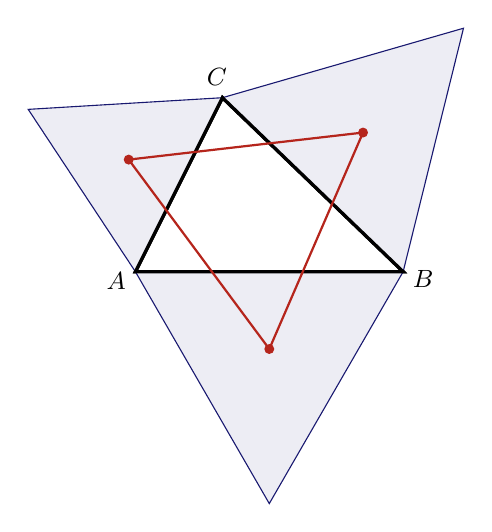
\begin{tikzpicture}[font=\small]
\draw[very thick] (0.0000,0.0000) -- (3.4000,0.0000) -- (1.1050,2.2100) -- cycle;
\draw[MidnightBlue,fill=MidnightBlue!8] (3.4000,0.0000) -- (4.1664,3.0925) -- (1.1050,2.2100) -- cycle;
\draw[MidnightBlue,fill=MidnightBlue!8] (1.1050,2.2100) -- (-1.3614,2.0620) -- (0.0000,0.0000) -- cycle;
\draw[MidnightBlue,fill=MidnightBlue!8] (0.0000,0.0000) -- (1.7000,-2.9445) -- (3.4000,0.0000) -- cycle;
\draw[very thick] (0.0000,0.0000) -- (3.4000,0.0000) -- (1.1050,2.2100) -- cycle;
\draw[BrickRed,thick] (2.8905,1.7675) -- (-0.0855,1.4240) -- (1.7000,-0.9815) -- cycle;
\fill[BrickRed] (2.8905,1.7675) circle (1.8pt);
\fill[BrickRed] (-0.0855,1.4240) circle (1.8pt);
\fill[BrickRed] (1.7000,-0.9815) circle (1.8pt);
\node at (-0.2442,-0.1198) {$A$};
\node at (3.6536,-0.0984) {$B$};
\node at (1.0343,2.4726) {$C$};
\end{tikzpicture}
